\section{Primera captura y análisis}
\par En esta primera instancia, vamos a correr nuestra herramienta para un destino en particular y analizaremos los resultados desde dos enfoques. Por una parte, veremos el recorrido de la ruta, los paises por los cuales pasa, el tiempo de respuesta de los distintos nodos y los saltos intercontinentales. Por otro lado, pondremos a prueba el funcionamiento de la herramienta y pensaremos en mejoras o correcciones que creamos pertinentes.

\subsection{Explicación del experimento}
\par Tomaremos como destino el host de la \textbf{Universidad de Ciudad del Cabo [uct.ac.za]}. Como mencionamos previamente, la herramienta irá aumentando el valor del campo \textit{ttl} hasta lograr una respuesta de la ip correspondiente a este host. Enviaremos 50 paquetes por cada valor de ttl, para obtener un buen promedio y evitar casos anormales.

\subsection{Resultados obtenidos}

\begin{figure}[ht]
  \begin{subfigure}[b]{.5\textwidth}
    \hspace*{-1.5cm}
    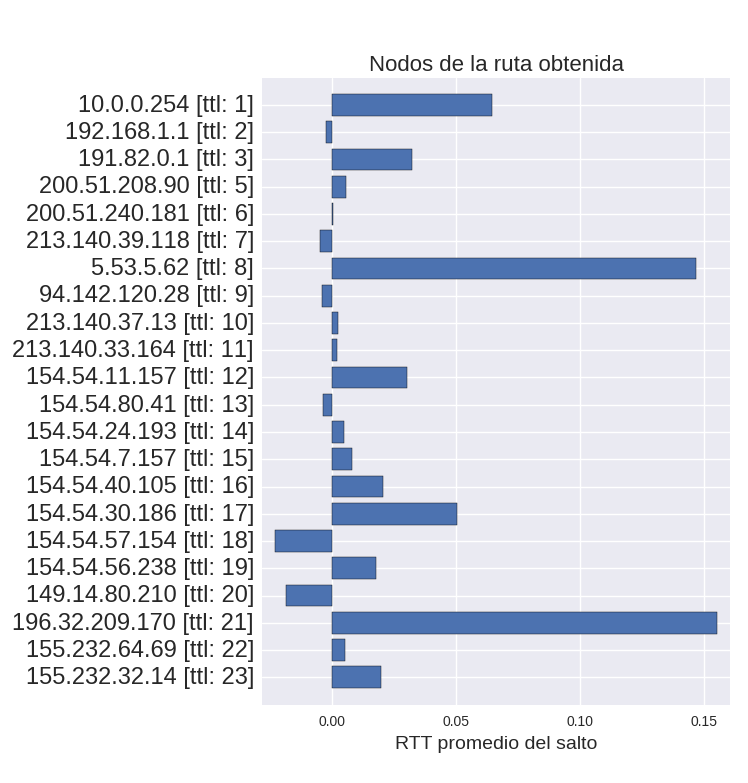
\includegraphics[width=1.2\textwidth]{Imagenes/capetown_rtts.png}
  \end{subfigure}
  \label{fig:capetown_rtts}
  \caption{Tiempo del salto entre cada nodo y su nodo previo, para cada nodo identificado en el camino al host uct.ac.za}
\end{figure}

\par En la figura \ref{fig:capetown_rtts} podemos ver el listado de nodos identificados en el camino al host destino y la comparación de los rtt promedio entre cada salto. Para cada nodo, se muestra el tiempo (promediado en segundos) que se tardó en llegar desde el nodo previo hasta él. Este valor se calcula tomando el tiempo que se tardó en llegar al nodo actual y restándole el mismo valor, pero del nodo previo.
\par Podemos ver que algunos valores de RTT resultan negativos. Esto se lo adjudicamos al hecho de que al recibir un paquete con ttl=0 algunos nodos tardan en enviar el paquete de respuesta (\textit{time exceded}), ya sea por restarle prioridad o por algún tema de procesamiento interno.
\par Otro dato importante que se observa de los resultados es que no se obtuvo el nodo con ttl=4. Creemos que esto se debe a que algunos nodos se encuentran configurados para no responder mensajes ICMP. En base a esto, tuvimos que tomar la determinación de ignorar los nodos que no respondan y suponer que los nodos previo y posterior se encuentran unidos. Esto influye fuértemente en el cálculo del tiempo de los saltos entre los nodos, ya que algunos saltos contienen en verdad algún nodo interno, el cual puede agregar tiempo.

\par En la figura \ref{fig:capetown_map} podemos ver la representación en un planisferio del camino recorrido hacia el destino, junto con la ubicación de los nodos intermedios. Se nota a simple vista lo poco intuitivo que resulta el camino. Pasa por España, Estados Unidos y Reino Unido, para luego llegar a Sudáfrica, donde se redirige a Ciudad del Cabo. Este fué uno de los motivos que nos llevó a elegir este host para ser analizado.

\begin{figure*}[ht]
  \hspace*{-0.4cm}
  \begin{subfigure}[b]{.60\textwidth}
    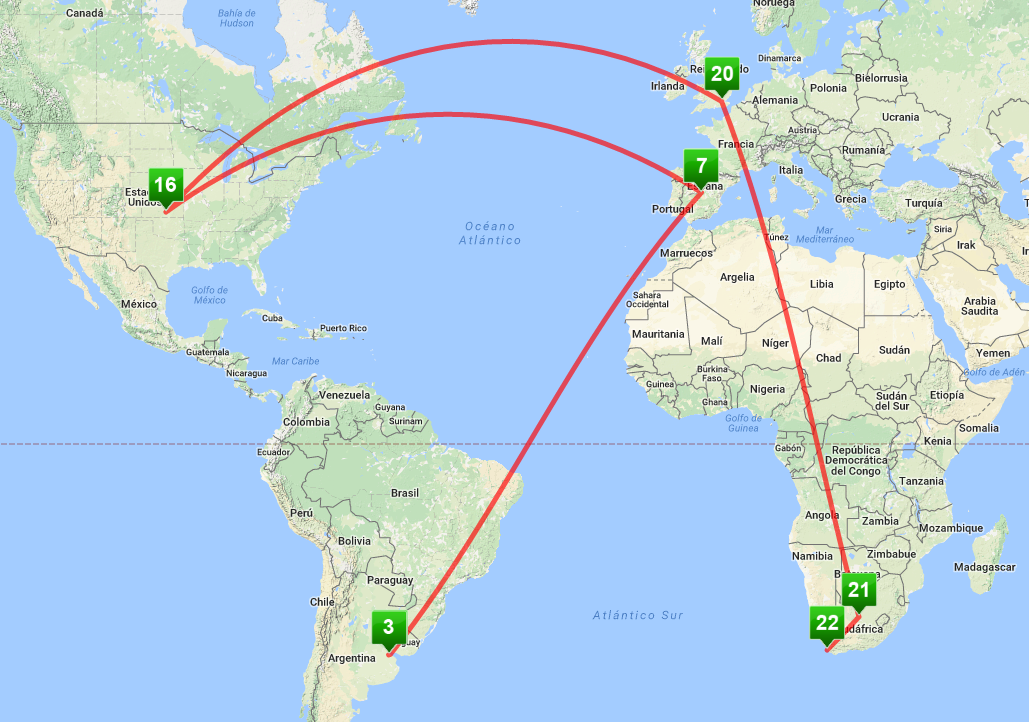
\includegraphics[width=\textwidth]{Imagenes/capetown_map.png}
    \label{fig:capetown_map}
    \caption{Mapa que muestra la unión de los nodos que forman el camino.}
  \end{subfigure}
  \begin{subfigure}[b]{.39\textwidth}
    \footnotesize
    \begin{tabular}{ l l l }
      \hline
      \textbf{TTL} & \textbf{IP} &  \textbf{País - Ciudad} \\ \hline
      1 & 10.0.0.254 &  - \\ \hline
      2 & 192.168.1.1 &  - \\ \hline
      3 & 191.82.0.1 & Argentina - Libertad\\ \hline
      5 & 200.51.208.90 & Argentina - \\ \hline
      6 & 200.51.240.181 & Argentina - \\ \hline
      7 & 213.140.39.118 & Spain - \\ \hline
      8 & 5.53.5.62 & Spain - \\ \hline
      9 & 94.142.120.28 & Spain - \\ \hline
      10 & 213.140.37.13 & Spain - \\ \hline
      11 & 213.140.33.164 & Spain - \\ \hline
      12 & 154.54.11.157 & United States - \\ \hline
      13 & 154.54.80.41 & United States - \\ \hline
      14 & 154.54.24.193 & United States - \\ \hline
      15 & 154.54.7.157 & United States - \\ \hline
      16 & 154.54.40.105 & United States - \\ \hline
      17 & 154.54.30.186 & United States - \\ \hline
      18 & 154.54.57.154 & United States - \\ \hline
      19 & 154.54.56.238 & United States - \\ \hline
      20 & 149.14.80.210 & United Kingdom - Mayfair\\ \hline
      21 & 196.32.209.170 & South Africa - \\ \hline
      22 & 155.232.64.69 & South Africa - Wynberg\\ \hline
      23 & 155.232.32.14 & South Africa - Wynberg\\ \hline
      \hline
    \end{tabular}
    \label{fig:capetown_list}
    \caption{Listado de nodos: TTL, IP y país.}
  \end{subfigure}
  \caption{Nodos pertenecientes al camino al host uct.ac.za.}
\end{figure*}
